\chapter{Revisão Bibliográfica e Fundamentação Teórica}\label{cap:cap2}

Este capítulo apresenta os conceitos necessários para o desenvolvimento da metodologia proposta. Inicialmente são discutidas as representações fasorial e sincrofasorial, pois elas definem a forma como sinais elétricos senoidais são descritos por magnitude e fase. Em seguida, são abordados os fasores harmônicos, as métricas de avaliação estabelecidas para PMUs e as limitações decorrentes de frequência variável. Por fim, são apresentados os fundamentos de interpolação B-Spline, estrutura de Farrow, filtros Flat-Top e decomposição polifásica, que formam a base técnica do método descrito no Capítulo~\ref{cap:tres}.

\section{Fasores}

Um fasor é uma representação complexa de uma grandeza senoidal em regime permanente. Essa representação é amplamente utilizada em sistemas elétricos porque permite substituir a descrição temporal completa de uma senoide por duas informações principais: magnitude e ângulo de fase. Com isso, a análise de circuitos e sistemas em corrente alternada torna-se mais simples, uma vez que a dependência temporal associada à frequência fundamental é separada da representação complexa da grandeza \cite{phadke2008}.

Considere o sinal senoidal

\begin{equation}
x(t) = X_m\cos(\omega t + \varphi),
\label{eq:cap2_sinal_senoidal}
\end{equation}

\noindent em que $X_m$ é a amplitude de pico, $\omega$ é a frequência angular e $\varphi$ é o ângulo de fase em relação a uma referência temporal. O valor eficaz associado à senoide é $X_m/\sqrt{2}$. Assim, o fasor correspondente pode ser escrito como

\begin{equation}
\bar{X} = \frac{X_m}{\sqrt{2}}e^{j\varphi}.
\label{eq:cap2_fasor}
\end{equation}

Na forma polar, a mesma grandeza é representada por

\begin{equation}
\bar{X} = X_{rms}\angle\varphi,
\label{eq:cap2_fasor_polar}
\end{equation}

\noindent em que $X_{rms}$ é o valor eficaz da grandeza. A informação temporal $\omega t$ não aparece explicitamente no fasor, pois a representação assume uma frequência de referência conhecida. Assim, o fasor convencional não descreve diretamente a evolução temporal do sinal; ele representa o módulo e o atraso angular da senoide em relação à referência adotada. Essa característica é adequada para regime permanente, mas torna-se mais delicada quando a frequência varia ao longo do tempo.

A Figura~\ref{fig:fasor} ilustra a relação entre uma senoide e sua representação no plano complexo. O ângulo do fasor indica a defasagem em relação à referência adotada, enquanto seu módulo está associado ao valor eficaz do sinal.

\begin{figure}[H]
    \centering
    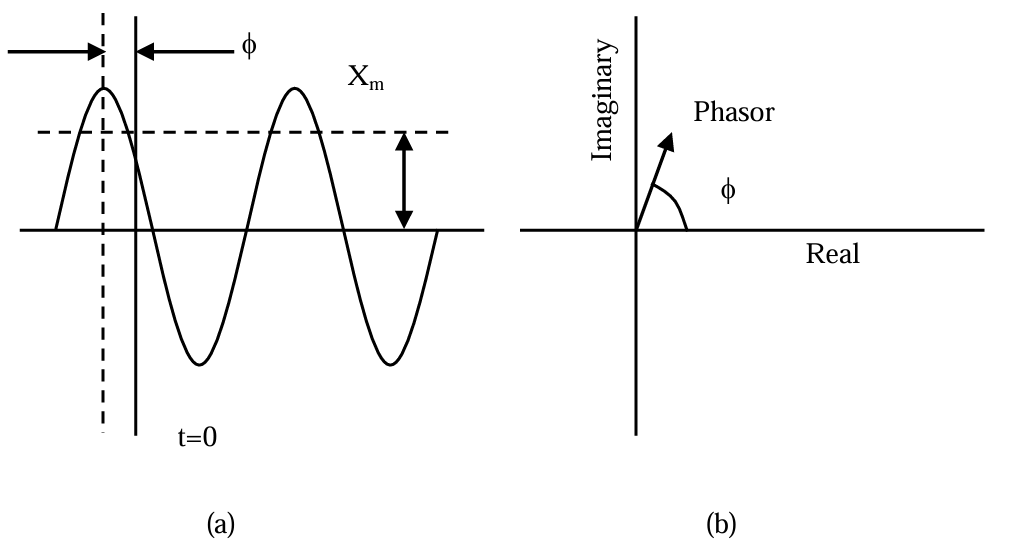
\includegraphics[scale=0.6]{textuais/capitulo2/imagens_capitulo_2/fasor_senoide.png}
    \caption{Representação de uma senoide e de seu fasor associado no plano complexo, adaptada de \cite{phadke2008}.}
    \label{fig:fasor}
\end{figure}

\section{Sincrofasores e PMUs}

Um sincrofasor é um fasor associado a uma referência temporal comum. Essa referência permite que medições realizadas em pontos geograficamente distintos de um sistema elétrico sejam comparadas de forma coerente. Em sistemas de medição fasorial sincronizada, essa base temporal é normalmente fornecida por sistemas de sincronização de alta precisão, como GPS, e utilizada por unidades de medição fasorial, conhecidas como PMUs (\textit{Phasor Measurement Units}) \cite{phadke2008,ieee2011}.

A principal diferença entre um fasor convencional e um sincrofasor está na associação explícita com uma estampa de tempo. Como o ângulo de fase depende do instante escolhido como referência, duas medições só podem ser comparadas de forma direta se estiverem sincronizadas. A vantagem prática dessa representação é permitir que fasores medidos em barras distintas sejam tratados como observações de um mesmo estado elétrico, preservando a coerência angular entre pontos afastados do sistema. Esse aspecto é fundamental em aplicações de monitoramento de grandes áreas, estimação de estado, proteção, controle e análise dinâmica de sistemas elétricos \cite{phadke2008,martins2012smfs}.

A Figura~\ref{fig:fasores_diversos} apresenta uma representação simplificada de medições fasoriais sincronizadas em diferentes pontos de um sistema elétrico. Na imagem, cada unidade de medição fornece um fasor local de tensão ou corrente, mas todos os ângulos são referidos à mesma base temporal. A existência dessa referência comum permite comparar os ângulos obtidos em barras distintas e relacioná-los ao estado operativo da rede.

\begin{figure}[H]
    \centering
    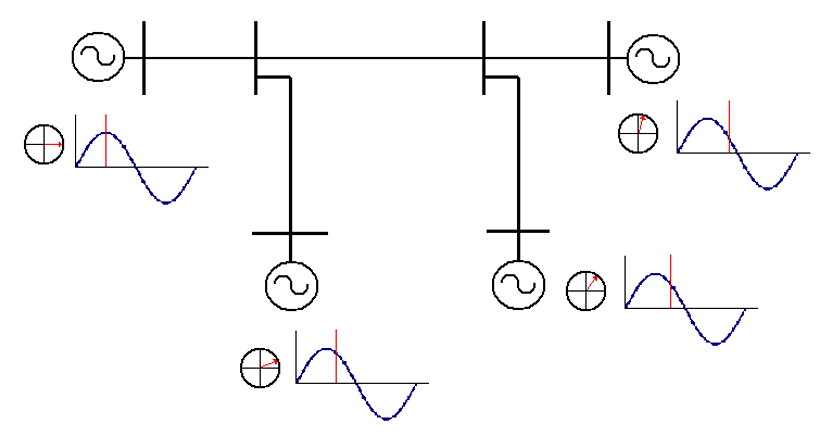
\includegraphics[scale=0.6]{textuais/capitulo2/imagens_capitulo_2/diferentes_fasores.png}
    \caption{Representação de medições fasoriais sincronizadas em diferentes pontos do sistema elétrico, adaptada de \cite{martins2012smfs}.}
    \label{fig:fasores_diversos}
\end{figure}

De forma geral, uma PMU realiza a aquisição dos sinais de tensão e corrente, aplica etapas de condicionamento e processamento digital, estima fasores, frequência e taxa de variação da frequência, e envia essas informações a um concentrador de dados fasoriais, ou PDC (\textit{Phasor Data Concentrator}). Esse arranjo é ilustrado na Figura~\ref{fig:PMU_max}.

\begin{figure}[H]
    \centering
    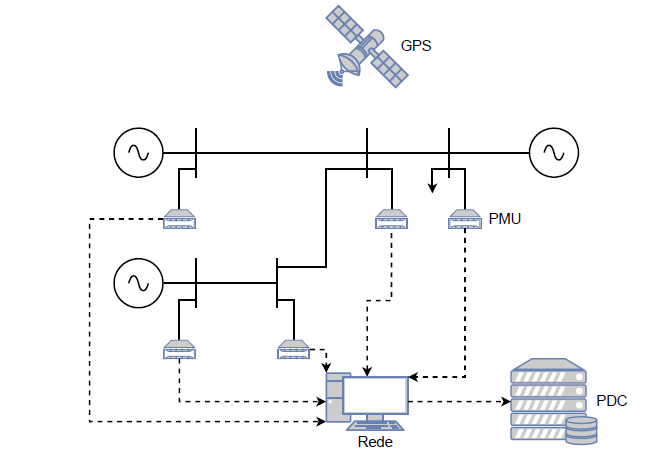
\includegraphics[scale=0.6]{textuais/capitulo2/imagens_capitulo_2/pmu_max.png}
    \caption{Estrutura geral de um sistema de medição fasorial sincronizada, adaptada de \cite{luiz2024qualificacao}.}
    \label{fig:PMU_max}
\end{figure}

\section{Estimação fasorial}

Na prática, os fasores não são obtidos a partir de expressões analíticas contínuas, mas por meio de sinais discretos adquiridos por conversores analógico-digitais. O problema da estimação fasorial consiste, portanto, em estimar magnitude, fase, frequência e, quando necessário, ROCOF a partir de um conjunto finito de amostras.

Entre as técnicas clássicas de estimação fasorial estão métodos baseados na DFT (\textit{Discrete Fourier Transform}), FFT (\textit{Fast Fourier Transform}), filtros digitais, PLLs, filtros de Kalman, métodos baseados em mínimos quadrados, Transformada de Taylor-Fourier e algoritmos interpolados no domínio da frequência. Cada família de métodos apresenta compromissos próprios entre precisão, tempo de resposta, robustez a ruído, rejeição de interferências e custo computacional.

Em condições estacionárias e com frequência nominal, métodos baseados na DFT tendem a apresentar boa precisão e implementação simples. Entretanto, quando a frequência do sinal se desvia da frequência nominal, a janela de observação deixa de conter um número inteiro de ciclos. Esse desalinhamento provoca espalhamento espectral e afeta a estimação da magnitude e da fase \cite{phadke2008,harris78}. O problema se torna ainda mais relevante em aplicações harmônicas, pois o erro de tempo ou de fase aparece no argumento das componentes em múltiplos da frequência fundamental. Assim, uma mesma incerteza angular associada à base temporal da fundamental tende a produzir efeito mais severo nas componentes de ordem elevada. Esse comportamento está no contexto dos desafios tratados em métodos de estimação de fasores harmônicos sob frequência variável \cite{duda2019,aleixo2022}.

Essa dificuldade pode ser vista diretamente a partir do referencial síncrono usado na definição fasorial. Considere uma senoide de valor eficaz $X_{\mathrm{rms}}$, frequência angular real $\omega$ e fase inicial $\varphi$,

\begin{equation}
x(t)=\sqrt{2}X_{\mathrm{rms}}\cos(\omega t+\varphi).
\label{eq:cap2_senoide_freq_real}
\end{equation}

\noindent Se a referência síncrona gira na frequência nominal $\omega_0$, a componente complexa associada ao sinal, observada nesse referencial, pode ser escrita como

\begin{equation}
\bar{X}(t)=X_{\mathrm{rms}}e^{j[(\omega-\omega_0)t+\varphi]}.
\label{eq:cap2_fasor_referencial_sincrono}
\end{equation}

\noindent Quando $\omega=\omega_0$, o termo dependente do tempo desaparece e o fasor permanece parado no referencial síncrono, com ângulo constante $\varphi$. Porém, quando $\omega\neq\omega_0$, surge uma rotação residual dada por

\begin{equation}
\varphi(t)=(\omega-\omega_0)t+\varphi.
\label{eq:cap2_fase_residual_freq}
\end{equation}

\noindent Portanto, a frequência fora da nominal não produz apenas um erro estático: ela faz o ângulo estimado variar ao longo da janela de observação. Em um estimador projetado para a base nominal, essa rotação residual aparece como deriva de fase e contribui para erros de magnitude e fase. Para componentes harmônicas, o mesmo raciocínio se torna mais crítico, pois a diferença angular é escalada pela ordem harmônica.

Esse contexto motiva o uso de técnicas que adaptem a análise à frequência real do sinal. Uma alternativa é reprojetar filtros sempre que a frequência muda. Outra possibilidade é reamostrar dinamicamente o sinal, de modo que o estimador posterior continue operando em uma base nominal. A metodologia deste trabalho segue a segunda abordagem, combinando estimação de frequência por cruzamento por zero e interpolação B-Spline para alimentar um banco de filtros harmônicos.

Nesse procedimento, as amostras originais continuam sendo adquiridas no relógio fixo do conversor analógico-digital. A partir dos cruzamentos por zero, estima-se o período elétrico real do sinal e calcula-se em quais instantes ele deveria ser observado para que cada ciclo fique compatível com a base nominal usada pelo estimador. Como esses instantes corrigidos geralmente caem entre duas amostras físicas, a interpolação B-Spline reconstrói o valor do sinal em posições fracionárias. Dessa forma, o método não altera o fenômeno medido; ele ajusta a base temporal entregue ao estimador. Uma componente que pareceria adiantada ou atrasada por causa do desvio de frequência passa a ser apresentada ao banco de filtros em instantes mais coerentes com a fase elétrica estimada. Os atrasos introduzidos pelos filtros e pelas etapas de média e interpolação são então compensados para que o fasor final permaneça referido ao instante correto.

\section{Fasores harmônicos}\label{sec:fasores_harmonicos}

Sinais elétricos reais podem conter componentes harmônicas decorrentes de cargas não lineares, conversores eletrônicos, saturação de equipamentos e outras fontes de distorção. Um sinal periódico não puramente senoidal pode ser representado como uma soma de componentes em múltiplos inteiros da frequência fundamental. Considerando uma frequência fundamental $f_1$, e seguindo a forma geral de sinais de ensaio adotada na IEC/IEEE 60255-118-1 \cite{iec60255}, uma representação simplificada é

\begin{equation}
x(t) = A_1\cos(2\pi f_1t + \varphi_1)
+ \sum_{h=2}^{H} A_h\cos(2\pi hf_1t + \varphi_h),
\label{eq:cap2_sinal_harmonicos}
\end{equation}

\noindent em que $h$ representa a ordem harmônica. O fasor associado à componente de ordem $h$ pode ser escrito como

\begin{equation}
\bar{X}_h = \frac{A_h}{\sqrt{2}}e^{j\varphi_h}.
\label{eq:cap2_fasor_harmonico}
\end{equation}

Quando a frequência fundamental varia, a fase da componente harmônica também passa a depender da trajetória temporal da frequência. Nesse caso, a fase instantânea da componente de ordem $h$ pode ser relacionada à fase da fundamental por

\begin{equation}
\theta_h(t) = h\theta_1(t) + \varphi_h.
\label{eq:cap2_fase_harmonico}
\end{equation}

Essa relação mostra por que a estimação de fasores harmônicos é sensível ao erro de frequência e ao desalinhamento temporal. Um pequeno erro na fase da componente fundamental tende a produzir erro proporcionalmente maior nas componentes de ordem elevada. Assim, técnicas de estimação harmônica precisam lidar simultaneamente com seletividade em frequência, precisão de fase e custo computacional.

A estimação sincronizada de fasores harmônicos ainda é um tema em desenvolvimento. Há aplicações potenciais em monitoramento de qualidade de energia, estimação de estado harmônico, localização de fontes de distorção, avaliação de filtros ativos e diagnóstico de fenômenos em redes com elevada penetração de eletrônica de potência. No entanto, diferentemente dos sincrofasores da componente fundamental, ainda não existe uma padronização ampla e consolidada para todos os requisitos de desempenho aplicáveis a HPMUs.

\section{Normas e métricas de avaliação}

As normas IEEE C37.118.1 e IEC/IEEE 60255-118-1 definem requisitos de desempenho para PMUs na estimação de sincrofasores, frequência e ROCOF da componente fundamental \cite{ieee2011,ieee2014,iec60255}. Essas normas estabelecem ensaios para condições estacionárias e dinâmicas, incluindo frequência fora da nominal, rampa de frequência, modulação de amplitude e modulação de fase.

Embora esses documentos não estabeleçam uma norma completa para fasores harmônicos, seus ensaios são úteis como referência metodológica. Neste trabalho, os cenários normativos são utilizados como base para construir sinais de teste contendo componentes harmônicas. Dessa forma, avalia-se o comportamento do método em condições compatíveis com aquelas usadas em PMUs, mas sem afirmar que a norma define todos os limites aplicáveis aos fasores harmônicos.

A métrica mais utilizada para avaliação fasorial é o TVE (\textit{Total Vector Error}), que compara o fasor estimado com o fasor de referência no plano complexo. Na IEC/IEEE 60255-118-1, essa métrica é definida por \cite{iec60255}

\begin{equation}
TVE =
100
\sqrt{
\frac{
\left(\hat{X}_r-X_r\right)^2+
\left(\hat{X}_i-X_i\right)^2
}{
X_r^2+X_i^2
}
},
\label{eq:cap2_tve}
\end{equation}

\noindent em que $\hat{X}_r$ e $\hat{X}_i$ são as partes real e imaginária do fasor estimado, e $X_r$ e $X_i$ são as partes real e imaginária do fasor de referência.

Além do TVE, a norma IEC/IEEE 60255-118-1 define o erro de frequência, dado por \cite{iec60255}

\begin{equation}
FE = \hat{f} - f,
\label{eq:cap2_fe}
\end{equation}

\noindent e o erro de ROCOF,

\begin{equation}
RFE = \widehat{ROCOF} - ROCOF.
\label{eq:cap2_rfe}
\end{equation}

Para interpretar o desempenho de estimadores harmônicos, também é útil separar o erro de magnitude e o erro de fase. O erro de magnitude indica a diferença entre os módulos dos fasores, enquanto o erro de fase indica o desalinhamento angular. Essa separação é importante porque dois estimadores podem apresentar TVE semelhante, mas por razões distintas: um pode ser limitado por erro de ganho, enquanto outro pode ser limitado por erro de fase.

\section{Interpolação e reamostragem dinâmica}

Uma estratégia para lidar com variação de frequência é reamostrar o sinal de entrada antes da estimação fasorial. A ideia é transformar uma sequência adquirida em taxa fixa em uma nova sequência cujos instantes estejam coerentes com a frequência estimada do sinal. Assim, em vez de alterar continuamente os filtros de extração harmônica, adapta-se a base temporal do sinal que alimenta esses filtros.

O ponto central é que a reamostragem não apenas aumenta ou reduz um buffer de amostras. Ela constrói uma nova grade de instantes para que o sinal seja observado de acordo com o período elétrico estimado. A fase inicial do sinal não é eliminada, pois ela faz parte do fasor que se deseja medir. O que se corrige é o descompasso acumulativo entre a grade temporal nominal e a frequência real do sinal. Em outras palavras, uma onda de \SI{61}{Hz} não deve ser forçada a ter fase de uma onda de \SI{60}{Hz}; ela deve ser entregue ao estimador em instantes tais que um ciclo real de \SI{61}{Hz} corresponda ao número nominal de amostras por ciclo usado pelo banco de filtros.

Considere que a taxa de aquisição seja $F_s=f_0N_{ppc}$, em que $N_{ppc}$ é o número nominal de pontos por ciclo. A aquisição original continua ocorrendo em taxa fixa, nos instantes $t_n=n/F_s$. A reamostragem não altera essa taxa de aquisição; ela apenas define uma nova grade de instantes $t_i[k]$ nos quais o sinal já adquirido será avaliado por interpolação.

Se o estimador posterior opera assumindo $N_{ppc}$ amostras por ciclo, então duas amostras consecutivas da sequência reamostrada devem estar separadas por $1/N_{ppc}$ do ciclo elétrico estimado. Como o período estimado é $1/\hat{f}[k]$, o avanço temporal desejado entre duas amostras interpoladas é

\begin{equation}
t_i[k+1] = t_i[k] + \frac{1}{N_{ppc}\hat{f}[k]}.
\label{eq:cap2_tempo_interpolado}
\end{equation}

\noindent Para implementar isso sobre o vetor discreto original, é conveniente trocar o tempo em segundos por uma posição em unidades de amostra original,

\begin{equation}
p_i[k] = F_s t_i[k].
\label{eq:cap2_posicao_interpolada}
\end{equation}

\noindent Assim, $p_i[k]$ indica onde a próxima saída interpolada deve ser calculada dentro da sequência original. Essa posição pode ser inteira ou fracionária. Substituindo \autoref{eq:cap2_tempo_interpolado} em \autoref{eq:cap2_posicao_interpolada}, obtém-se

\begin{equation}
p_i[k+1] = p_i[k] + \lambda[k],
\qquad
\lambda[k] = \frac{F_s}{N_{ppc}\hat{f}[k]} = \frac{f_0}{\hat{f}[k]}.
\label{eq:cap2_lambda}
\end{equation}

\noindent Portanto, $\lambda[k]$ é o passo da posição temporal do interpolador. Ele não multiplica a amplitude da amostra. Para calcular a saída, toma-se a parte inteira $n_k=\lfloor p_i[k]\rfloor$ e a parte fracionária $\alpha_k=p_i[k]-n_k$. O interpolador B-Spline usa $\alpha_k$ e as amostras vizinhas armazenadas no buffer para estimar o valor do sinal naquele instante fracionário.

Quando $\hat{f}>f_0$, tem-se $\lambda<1$. Nesse caso, cada nova amostra interpolada avança menos de uma amostra no eixo da sequência original. Isso ocorre porque o ciclo real é mais curto e, na sequência original, contém menos do que $N_{ppc}$ amostras físicas. Por exemplo, para $f_0=\SI{60}{Hz}$ e $\hat{f}=\SI{61}{Hz}$, um ciclo real ocupa aproximadamente $(60/61)N_{ppc}$ amostras originais. Com $\lambda=60/61$, após gerar $N_{ppc}$ amostras interpoladas, a posição $p_i[k]$ terá avançado exatamente esse intervalo, isto é, um ciclo elétrico estimado.

Quando $\hat{f}<f_0$, tem-se $\lambda>1$. Nesse caso, cada nova amostra interpolada avança mais de uma amostra no eixo original, pois o ciclo real é mais longo e contém mais do que $N_{ppc}$ amostras físicas. Assim, a reamostragem não muda a taxa do conversor A/D; ela muda apenas os instantes, representados por $p_i[k]$, em que o sinal armazenado no buffer é avaliado. O objetivo é entregar ao banco de filtros uma sequência na qual um ciclo elétrico estimado corresponda novamente a $N_{ppc}$ amostras.

Desse modo, a discrepância de frequência não é ignorada; ela é usada para escolher os instantes de interpolação. O erro que se busca reduzir é a deriva de fase causada por aplicar uma grade nominal fixa a um sinal cujo período real é diferente. O sucesso desse procedimento depende diretamente da qualidade da estimativa de frequência, da precisão do interpolador e da compensação dos atrasos introduzidos pelos filtros e médias usados antes da extração fasorial.

\section{Interpolação B-Spline e estrutura de Farrow}

As B-Splines são funções de base utilizadas em problemas de aproximação e interpolação, com propriedades de suavidade e suporte compacto \cite{uns99}. No contexto de estimação fasorial harmônica, a interpolação B-Spline é empregada para gerar amostras em instantes fracionários, permitindo a reamostragem dinâmica do sinal em função da frequência estimada \cite{aleixo2022,aleixoTese}.

Na forma cúbica, a interpolação pode ser implementada de maneira eficiente por uma estrutura de Farrow. Essa estrutura representa o interpolador como uma combinação polinomial de subfiltros fixos, forma usual para implementar atrasos fracionários variáveis sem alterar continuamente os coeficientes internos do filtro \cite{aleixo2022,aleixoTese}. Para um parâmetro fracionário $\alpha$, a saída interpolada pode ser escrita de forma geral como

\begin{equation}
y[n,\alpha] = \sum_{p=0}^{P} H_p[n]\alpha^p,
\label{eq:cap2_farrow_geral}
\end{equation}

\noindent em que $H_p[n]$ são as saídas dos subfiltros e $P$ é a ordem do polinômio. No caso cúbico, $P=3$. A principal vantagem dessa estrutura, já explorada em interpoladores para estimação fasorial, é que os coeficientes dos subfiltros permanecem fixos, enquanto o atraso fracionário é ajustado apenas pelo parâmetro $\alpha$. Isso evita o reprojeto do filtro a cada nova frequência estimada \cite{aleixo2022,aleixoTese}.

Como a interpolação B-Spline cúbica não é naturalmente interpolante em todos os pontos amostrados, utiliza-se um pré-filtro para obter os coeficientes adequados da expansão. Esse pré-filtro compensa a suavização da base B-Spline e melhora a preservação das componentes do sinal. Para estimação harmônica, essa compensação é relevante porque pequenas alterações de amplitude e fase podem ser amplificadas nas componentes de ordem elevada.

\section{Filtros Flat-Top}

Filtros e janelas Flat-Top são projetados para apresentar resposta de magnitude muito plana em torno da frequência central. Essa propriedade é desejável quando o objetivo é estimar amplitudes com baixa sensibilidade a pequenos desvios de frequência \cite{harris78,duda2016}. Em estimação de fasores harmônicos, filtros Flat-Top têm sido utilizados por sua capacidade de reduzir erro de amplitude e preservar a informação de fase dentro da banda de interesse \cite{duda2016,duda2019}.

Um filtro Flat-Top pode ser construído a partir de uma combinação de cossenos, como

\begin{equation}
w[n] = \sum_{m=0}^{P} a_m \cos\left(\frac{2\pi mn}{N}\right),
\label{eq:cap2_flattop}
\end{equation}

\noindent seguida de normalização adequada. A partir do filtro protótipo, filtros centrados em diferentes frequências podem ser obtidos por modulação complexa. Quando essa estratégia é aplicada a várias componentes harmônicas, obtém-se um banco de filtros.

O uso direto de um filtro para cada componente pode exigir elevado número de operações, principalmente quando muitas ordens harmônicas são estimadas simultaneamente. A partir das propriedades dos filtros Flat-Top e da teoria de bancos polifásicos, a combinação entre essas técnicas torna-se atrativa: preserva as propriedades de estimação do filtro protótipo e reduz a carga computacional associada ao banco \cite{duda2019,mk06}.

\section{Decomposição polifásica e bancos de filtros}

A decomposição polifásica é uma ferramenta clássica de processamento multitaxa. Ela permite reescrever um filtro em componentes que operam em fases distintas da sequência de entrada, possibilitando implementações eficientes de decimadores, interpoladores e bancos de filtros \cite{mk06}. Para um filtro $H(z)$, a decomposição polifásica do Tipo I é dada por

\begin{equation}
H(z) = \sum_{\ell=0}^{M-1} z^{-\ell}E_{\ell}(z^M),
\label{eq:cap2_polifasica}
\end{equation}

\noindent em que $M$ é o número de fases e $E_{\ell}(z)$ são os componentes polifásicos.

Em um banco de filtros uniforme, o filtro protótipo é deslocado em frequência para formar múltiplos canais. A implementação direta requer a filtragem individual de cada canal. Na forma polifásica, a filtragem é reorganizada em taxa reduzida e combinada com uma DFT ou IFFT, reduzindo o número de operações. Para um filtro protótipo com $N$ coeficientes e um banco com $M$ canais, a complexidade aproximada pode ser reduzida de uma ordem proporcional a $NM$ para uma ordem proporcional a

\begin{equation}
N + M\log_2(M).
\label{eq:cap2_complexidade}
\end{equation}

Essa redução é um dos elementos centrais deste trabalho. Como a estimação de fasores harmônicos pode exigir dezenas de canais, a forma polifásica contribui para tornar o método mais adequado a aplicações em tempo real e a implementações embarcadas. A metodologia proposta no Capítulo~\ref{cap:tres} utiliza essa estrutura para organizar o banco Flat-Top de forma computacionalmente eficiente.

\section{Considerações finais do capítulo}

Este capítulo apresentou os fundamentos necessários para compreender a metodologia proposta. A representação fasorial define o objeto de estimação; os sincrofasores e as normas de PMUs fornecem o contexto de avaliação; a discussão sobre fasores harmônicos evidencia a dificuldade adicional causada pela multiplicação dos erros de fase; e os conceitos de interpolação B-Spline, Farrow, filtros Flat-Top e decomposição polifásica formam a base do método desenvolvido.

No capítulo seguinte, esses elementos são combinados em uma cadeia de processamento única, voltada à estimação de fasores harmônicos em condições de frequência variável. A ênfase passa então da fundamentação individual de cada técnica para a forma como elas são integradas no algoritmo proposto.
